% Created by tikzDevice version 0.12.3.1 on 2022-09-01 15:50:29
% !TEX encoding = UTF-8 Unicode
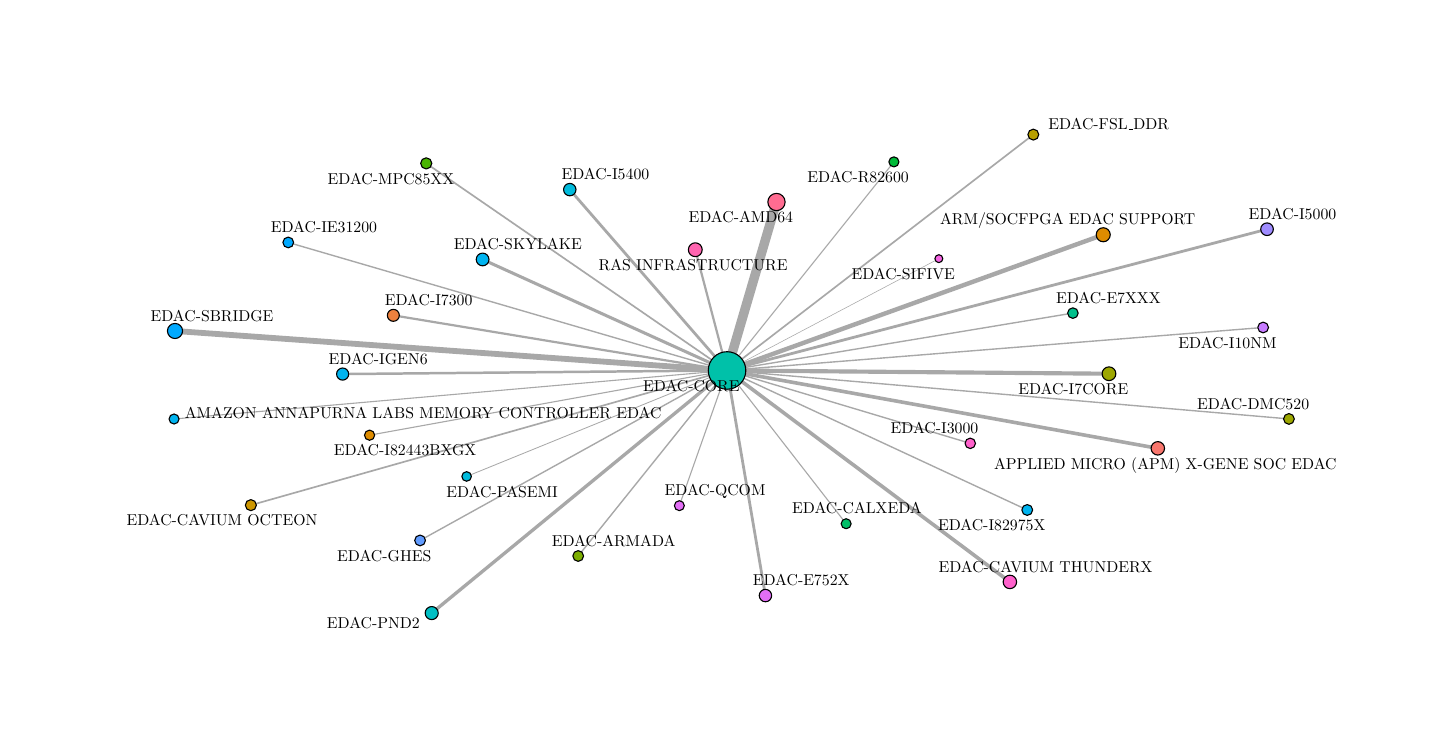
\begin{tikzpicture}[x=1pt,y=1pt]
\definecolor{fillColor}{RGB}{255,255,255}
\path[use as bounding box,fill=fillColor,fill opacity=0.00] (0,0) rectangle (505.89,252.94);
\begin{scope}
\path[clip] (  0.00,  0.00) rectangle (505.89,252.94);
\definecolor{fillColor}{RGB}{255,255,255}

\path[fill=fillColor] (  0.00,  0.00) rectangle (505.89,252.94);
\end{scope}
\begin{scope}
\path[clip] ( 32.75, 32.75) rectangle (475.89,222.94);
\definecolor{drawColor}{gray}{0.66}

\path[draw=drawColor,line width= 0.4pt,line join=round] ( 52.89,111.53) -- (252.72,129.07);

\path[draw=drawColor,line width= 1.3pt,line join=round] (408.37,100.93) -- (252.72,129.07);

\path[draw=drawColor,line width= 1.6pt,line join=round] (388.65,178.11) -- (252.72,129.07);

\path[draw=drawColor,line width= 3.4pt,line join=round] (270.58,189.94) -- (252.72,129.07);

\path[draw=drawColor,line width= 0.5pt,line join=round] (198.93, 62.03) -- (252.72,129.07);

\path[draw=drawColor,line width= 0.4pt,line join=round] (295.75, 73.69) -- (252.72,129.07);

\path[draw=drawColor,line width= 0.6pt,line join=round] ( 80.65, 80.40) -- (252.72,129.07);

\path[draw=drawColor,line width= 1.3pt,line join=round] (354.92, 52.66) -- (252.72,129.07);

\path[draw=drawColor,line width= 0.5pt,line join=round] (252.72,129.07) -- (455.75,111.56);

\path[draw=drawColor,line width= 1.0pt,line join=round] (252.72,129.07) -- (266.59, 47.73);

\path[draw=drawColor,line width= 0.5pt,line join=round] (252.72,129.07) -- (377.69,149.80);

\path[draw=drawColor,line width= 0.6pt,line join=round] (252.72,129.07) -- (363.39,214.30);

\path[draw=drawColor,line width= 0.5pt,line join=round] (252.72,129.07) -- (141.79, 67.65);

\path[draw=drawColor,line width= 0.5pt,line join=round] (252.72,129.07) -- (446.43,144.60);

\path[draw=drawColor,line width= 0.5pt,line join=round] (252.72,129.07) -- (340.60,102.74);

\path[draw=drawColor,line width= 1.0pt,line join=round] (252.72,129.07) -- (447.84,180.11);

\path[draw=drawColor,line width= 1.0pt,line join=round] (252.72,129.07) -- (195.89,194.42);

\path[draw=drawColor,line width= 0.8pt,line join=round] (252.72,129.07) -- (132.13,148.99);

\path[draw=drawColor,line width= 1.5pt,line join=round] (252.72,129.07) -- (390.73,127.89);

\path[draw=drawColor,line width= 0.4pt,line join=round] (252.72,129.07) -- (123.54,105.68);

\path[draw=drawColor,line width= 0.5pt,line join=round] (252.72,129.07) -- (361.19, 78.66);

\path[draw=drawColor,line width= 0.5pt,line join=round] (252.72,129.07) -- ( 94.16,175.33);

\path[draw=drawColor,line width= 0.9pt,line join=round] (252.72,129.07) -- (113.81,127.77);

\path[draw=drawColor,line width= 0.6pt,line join=round] (252.72,129.07) -- (144.02,203.90);

\path[draw=drawColor,line width= 0.3pt,line join=round] (252.72,129.07) -- (158.61, 90.77);

\path[draw=drawColor,line width= 1.2pt,line join=round] (252.72,129.07) -- (146.00, 41.40);

\path[draw=drawColor,line width= 0.4pt,line join=round] (252.72,129.07) -- (235.48, 80.21);

\path[draw=drawColor,line width= 0.4pt,line join=round] (252.72,129.07) -- (313.01,204.44);

\path[draw=drawColor,line width= 2.1pt,line join=round] (252.72,129.07) -- ( 53.24,143.34);

\path[draw=drawColor,line width= 0.2pt,line join=round] (252.72,129.07) -- (329.25,169.47);

\path[draw=drawColor,line width= 1.1pt,line join=round] (252.72,129.07) -- (164.39,169.18);

\path[draw=drawColor,line width= 0.8pt,line join=round] (252.72,129.07) -- (241.24,172.70);
\definecolor{drawColor}{RGB}{0,0,0}
\definecolor{fillColor}{RGB}{0,180,240}

\path[draw=drawColor,line width= 0.4pt,line join=round,line cap=round,fill=fillColor] ( 52.89,111.53) circle (  1.81);
\definecolor{fillColor}{RGB}{248,118,109}

\path[draw=drawColor,line width= 0.4pt,line join=round,line cap=round,fill=fillColor] (408.37,100.93) circle (  2.43);
\definecolor{fillColor}{RGB}{222,140,0}

\path[draw=drawColor,line width= 0.4pt,line join=round,line cap=round,fill=fillColor] (388.65,178.11) circle (  2.53);
\definecolor{fillColor}{RGB}{255,108,145}

\path[draw=drawColor,line width= 0.4pt,line join=round,line cap=round,fill=fillColor] (270.58,189.94) circle (  3.12);
\definecolor{fillColor}{RGB}{124,174,0}

\path[draw=drawColor,line width= 0.4pt,line join=round,line cap=round,fill=fillColor] (198.93, 62.03) circle (  1.94);
\definecolor{fillColor}{RGB}{0,190,103}

\path[draw=drawColor,line width= 0.4pt,line join=round,line cap=round,fill=fillColor] (295.75, 73.69) circle (  1.81);
\definecolor{fillColor}{RGB}{205,150,0}

\path[draw=drawColor,line width= 0.4pt,line join=round,line cap=round,fill=fillColor] ( 80.65, 80.40) circle (  2.00);
\definecolor{fillColor}{RGB}{255,97,204}

\path[draw=drawColor,line width= 0.4pt,line join=round,line cap=round,fill=fillColor] (354.92, 52.66) circle (  2.43);
\definecolor{fillColor}{RGB}{0,193,169}

\path[draw=drawColor,line width= 0.4pt,line join=round,line cap=round,fill=fillColor] (252.72,129.07) circle (  6.78);
\definecolor{fillColor}{RGB}{157,167,0}

\path[draw=drawColor,line width= 0.4pt,line join=round,line cap=round,fill=fillColor] (455.75,111.56) circle (  1.94);
\definecolor{fillColor}{RGB}{227,110,246}

\path[draw=drawColor,line width= 0.4pt,line join=round,line cap=round,fill=fillColor] (266.59, 47.73) circle (  2.24);
\definecolor{fillColor}{RGB}{0,192,139}

\path[draw=drawColor,line width= 0.4pt,line join=round,line cap=round,fill=fillColor] (377.69,149.80) circle (  1.91);
\definecolor{fillColor}{RGB}{183,159,0}

\path[draw=drawColor,line width= 0.4pt,line join=round,line cap=round,fill=fillColor] (363.39,214.30) circle (  1.97);
\definecolor{fillColor}{RGB}{97,156,255}

\path[draw=drawColor,line width= 0.4pt,line join=round,line cap=round,fill=fillColor] (141.79, 67.65) circle (  1.95);
\definecolor{fillColor}{RGB}{199,124,255}

\path[draw=drawColor,line width= 0.4pt,line join=round,line cap=round,fill=fillColor] (446.43,144.60) circle (  1.94);
\definecolor{fillColor}{RGB}{255,97,204}

\path[draw=drawColor,line width= 0.4pt,line join=round,line cap=round,fill=fillColor] (340.60,102.74) circle (  1.89);
\definecolor{fillColor}{RGB}{159,140,255}

\path[draw=drawColor,line width= 0.4pt,line join=round,line cap=round,fill=fillColor] (447.84,180.11) circle (  2.28);
\definecolor{fillColor}{RGB}{0,187,220}

\path[draw=drawColor,line width= 0.4pt,line join=round,line cap=round,fill=fillColor] (195.89,194.42) circle (  2.24);
\definecolor{fillColor}{RGB}{237,129,62}

\path[draw=drawColor,line width= 0.4pt,line join=round,line cap=round,fill=fillColor] (132.13,148.99) circle (  2.16);
\definecolor{fillColor}{RGB}{157,167,0}

\path[draw=drawColor,line width= 0.4pt,line join=round,line cap=round,fill=fillColor] (390.73,127.89) circle (  2.48);
\definecolor{fillColor}{RGB}{222,140,0}

\path[draw=drawColor,line width= 0.4pt,line join=round,line cap=round,fill=fillColor] (123.54,105.68) circle (  1.84);
\definecolor{fillColor}{RGB}{0,180,240}

\path[draw=drawColor,line width= 0.4pt,line join=round,line cap=round,fill=fillColor] (361.19, 78.66) circle (  1.96);
\definecolor{fillColor}{RGB}{0,169,255}

\path[draw=drawColor,line width= 0.4pt,line join=round,line cap=round,fill=fillColor] ( 94.16,175.33) circle (  1.94);
\definecolor{fillColor}{RGB}{0,180,240}

\path[draw=drawColor,line width= 0.4pt,line join=round,line cap=round,fill=fillColor] (113.81,127.77) circle (  2.19);
\definecolor{fillColor}{RGB}{73,181,0}

\path[draw=drawColor,line width= 0.4pt,line join=round,line cap=round,fill=fillColor] (144.02,203.90) circle (  2.02);
\definecolor{fillColor}{RGB}{0,187,220}

\path[draw=drawColor,line width= 0.4pt,line join=round,line cap=round,fill=fillColor] (158.61, 90.77) circle (  1.73);
\definecolor{fillColor}{RGB}{0,191,196}

\path[draw=drawColor,line width= 0.4pt,line join=round,line cap=round,fill=fillColor] (146.00, 41.40) circle (  2.36);
\definecolor{fillColor}{RGB}{227,110,246}

\path[draw=drawColor,line width= 0.4pt,line join=round,line cap=round,fill=fillColor] (235.48, 80.21) circle (  1.80);
\definecolor{fillColor}{RGB}{0,186,56}

\path[draw=drawColor,line width= 0.4pt,line join=round,line cap=round,fill=fillColor] (313.01,204.44) circle (  1.82);
\definecolor{fillColor}{RGB}{0,169,255}

\path[draw=drawColor,line width= 0.4pt,line join=round,line cap=round,fill=fillColor] ( 53.24,143.34) circle (  2.73);
\definecolor{fillColor}{RGB}{245,100,227}

\path[draw=drawColor,line width= 0.4pt,line join=round,line cap=round,fill=fillColor] (329.25,169.47) circle (  1.43);
\definecolor{fillColor}{RGB}{0,180,240}

\path[draw=drawColor,line width= 0.4pt,line join=round,line cap=round,fill=fillColor] (164.39,169.18) circle (  2.30);
\definecolor{fillColor}{RGB}{255,100,176}

\path[draw=drawColor,line width= 0.4pt,line join=round,line cap=round,fill=fillColor] (241.24,172.70) circle (  2.50);

\node[text=drawColor,anchor=base,inner sep=0pt, outer sep=0pt, scale=  0.57] at (142.91,111.61) {AMAZON ANNAPURNA LABS MEMORY CONTROLLER EDAC};

\node[text=drawColor,anchor=base,inner sep=0pt, outer sep=0pt, scale=  0.57] at (411.08, 93.46) {APPLIED MICRO (APM) X-GENE SOC EDAC};

\node[text=drawColor,anchor=base,inner sep=0pt, outer sep=0pt, scale=  0.57] at (375.81,181.67) {ARM/SOCFPGA EDAC SUPPORT};

\node[text=drawColor,anchor=base,inner sep=0pt, outer sep=0pt, scale=  0.57] at (257.72,182.44) {EDAC-AMD64};

\node[text=drawColor,anchor=base,inner sep=0pt, outer sep=0pt, scale=  0.57] at (211.75, 65.58) {EDAC-ARMADA};

\node[text=drawColor,anchor=base,inner sep=0pt, outer sep=0pt, scale=  0.57] at (299.67, 77.28) {EDAC-CALXEDA};

\node[text=drawColor,anchor=base,inner sep=0pt, outer sep=0pt, scale=  0.57] at ( 70.20, 72.93) {EDAC-CAVIUM OCTEON};

\node[text=drawColor,anchor=base,inner sep=0pt, outer sep=0pt, scale=  0.57] at (367.81, 56.24) {EDAC-CAVIUM THUNDERX};

\node[text=drawColor,anchor=base,inner sep=0pt, outer sep=0pt, scale=  0.57] at (239.83,121.57) {EDAC-CORE};

\node[text=drawColor,anchor=base,inner sep=0pt, outer sep=0pt, scale=  0.57] at (442.83,115.12) {EDAC-DMC520};

\node[text=drawColor,anchor=base,inner sep=0pt, outer sep=0pt, scale=  0.57] at (279.51, 51.31) {EDAC-E752X};

\node[text=drawColor,anchor=base,inner sep=0pt, outer sep=0pt, scale=  0.57] at (390.51,153.36) {EDAC-E7XXX};

\node[text=drawColor,anchor=base,inner sep=0pt, outer sep=0pt, scale=  0.57] at (390.62,216.01) {EDAC-FSL{\_{}}DDR};

\node[text=drawColor,anchor=base,inner sep=0pt, outer sep=0pt, scale=  0.57] at (128.86, 60.16) {EDAC-GHES};

\node[text=drawColor,anchor=base,inner sep=0pt, outer sep=0pt, scale=  0.57] at (433.57,137.12) {EDAC-I10NM};

\node[text=drawColor,anchor=base,inner sep=0pt, outer sep=0pt, scale=  0.57] at (327.69,106.32) {EDAC-I3000};

\node[text=drawColor,anchor=base,inner sep=0pt, outer sep=0pt, scale=  0.57] at (457.04,183.67) {EDAC-I5000};

\node[text=drawColor,anchor=base,inner sep=0pt, outer sep=0pt, scale=  0.57] at (208.78,197.99) {EDAC-I5400};

\node[text=drawColor,anchor=base,inner sep=0pt, outer sep=0pt, scale=  0.57] at (144.91,152.53) {EDAC-I7300};

\node[text=drawColor,anchor=base,inner sep=0pt, outer sep=0pt, scale=  0.57] at (377.85,120.40) {EDAC-I7CORE};

\node[text=drawColor,anchor=base,inner sep=0pt, outer sep=0pt, scale=  0.57] at (136.37, 98.21) {EDAC-I82443BXGX};

\node[text=drawColor,anchor=base,inner sep=0pt, outer sep=0pt, scale=  0.57] at (348.38, 71.18) {EDAC-I82975X};

\node[text=drawColor,anchor=base,inner sep=0pt, outer sep=0pt, scale=  0.57] at (107.08,178.92) {EDAC-IE31200};

\node[text=drawColor,anchor=base,inner sep=0pt, outer sep=0pt, scale=  0.57] at (126.66,131.34) {EDAC-IGEN6};

\node[text=drawColor,anchor=base,inner sep=0pt, outer sep=0pt, scale=  0.57] at (131.25,196.45) {EDAC-MPC85XX};

\node[text=drawColor,anchor=base,inner sep=0pt, outer sep=0pt, scale=  0.57] at (171.43, 83.30) {EDAC-PASEMI};

\node[text=drawColor,anchor=base,inner sep=0pt, outer sep=0pt, scale=  0.57] at (124.94, 35.76) {EDAC-PND2};

\node[text=drawColor,anchor=base,inner sep=0pt, outer sep=0pt, scale=  0.57] at (248.40, 83.80) {EDAC-QCOM};

\node[text=drawColor,anchor=base,inner sep=0pt, outer sep=0pt, scale=  0.57] at (300.10,196.94) {EDAC-R82600};

\node[text=drawColor,anchor=base,inner sep=0pt, outer sep=0pt, scale=  0.57] at ( 66.62,146.91) {EDAC-SBRIDGE};

\node[text=drawColor,anchor=base,inner sep=0pt, outer sep=0pt, scale=  0.57] at (316.38,162.00) {EDAC-SIFIVE};

\node[text=drawColor,anchor=base,inner sep=0pt, outer sep=0pt, scale=  0.57] at (177.12,172.73) {EDAC-SKYLAKE};

\node[text=drawColor,anchor=base,inner sep=0pt, outer sep=0pt, scale=  0.57] at (240.46,165.25) {RAS INFRASTRUCTURE};
\end{scope}
\end{tikzpicture}
